\chapter{综述}
\label{chap2}

\section{问题综述}
在计算路况时,由于数据的稀疏性,会出现两个GPS坐标之间相隔一个路口甚至更多的情况,但是我们要分别统计每一段路的路况,所以要把两段道路的路况进行分离。建立模型时把每段轨迹的时间分成两段路的用时加上虚拟的路口转向延迟三个部分,对于每个路段,如果存在正反两个方向则两个方向的路况互不干扰单独计算。

拿十字路口举例,如图~\ref{fig:1}所示,一个路口的参数包含4个路段每个路段两个方向共8个方向的路况参数,路口12个方向的转向延迟。当前系统的处理方式是直接把每段轨迹的时间按照经过道路的长度加权分配在每段路上,再由通过同一路段的所有轨迹加权得到该路段的用时,推算出平均速度来表示路况。

\begin{figure}[H] 
  \centering
  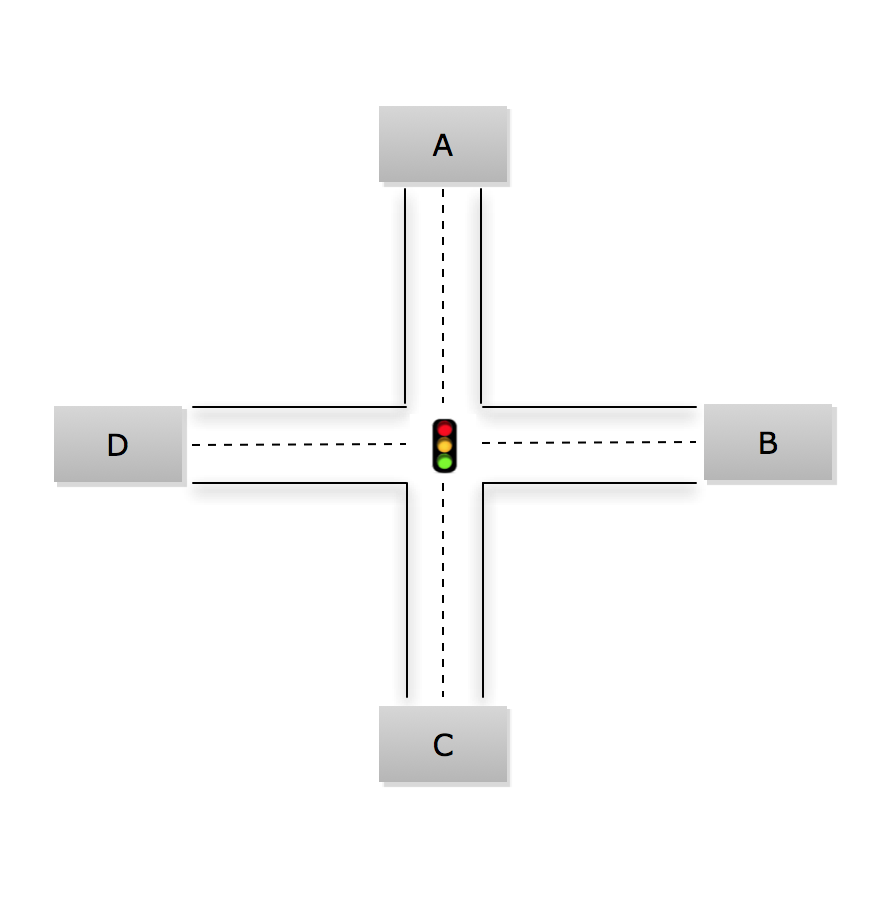
\includegraphics[width=3.5in]{intersection}
  \caption{路口示意图}
  \label{fig:1}
\end{figure}

拿AB段举例,将路口设为O点,这时如果出现AO段行驶畅通而OB段堵塞的情况,时间会平摊到AO和OB两段,这样计算出的结果不能反映真实的路况。又考虑到一定时间内路况不出现大的变化,本文的算法选取一定时间内通过同一路口的数据,使用这些数据直接计算出每一段的精确路况,从而能够更准确地反映每段路分别的路况信息。


\section{相关工作}
\label{sec:related_work}

\subsection{平滑算法}

\begin{figure}[H] 
  \centering
  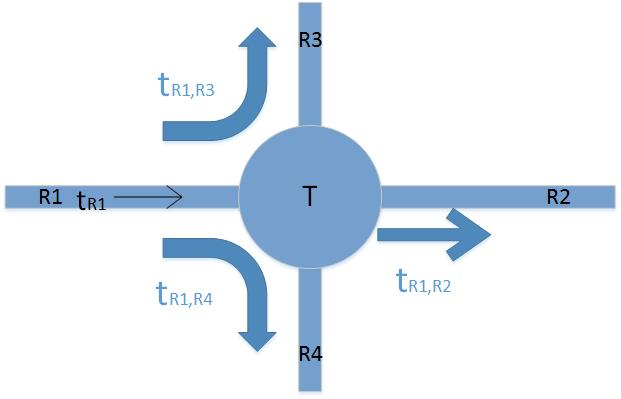
\includegraphics[width=3in]{road_model}
  \caption{平滑算法}
  \label{fig:2}
\end{figure}

该算法中跨路口的轨迹,如图~\ref{fig:2}所示,拿$R1\to R2$举例,包括前一段路R1的行驶时间$t_{R1}$,转向延迟$t_{R1,R2}$和第二段路的行驶时间$t_{R2}$(\ref{f2.1.1})。然后计算当前道路的通过时间以及到下一条道路的转向时间的和在总时间中的比重(\ref{f2.1.2})。之后计算实际花费的时间(\ref{f2.1.3})。最后按比例分配行驶时间与转向时间(\ref{f2.1.4})。这种做法优势是实现起来非常简单,通用性强,但是对于某些路况分布不均匀情况可能效果不是很理想。

\begin{equation}
t=t_{R1}+t_{R1,R2}+t_{R2}
\label{f2.1.1}
\end{equation}
\begin{equation}
percentage = (cover\_rate\times road\_length/road\_speed + turn\_time) / total\_time;
\label{f2.1.2}
\end{equation}
\begin{equation}
real\_time = interval\times percentage;
\label{f2.1.3}
\end{equation}
\begin{equation}
turn\_delay = real\_time \times turn\_time/(turn\_time + trip\_time);
\label{f2.1.4}
\end{equation}

\subsection{路段分解算法}

\begin{figure}[H] 
  \centering
  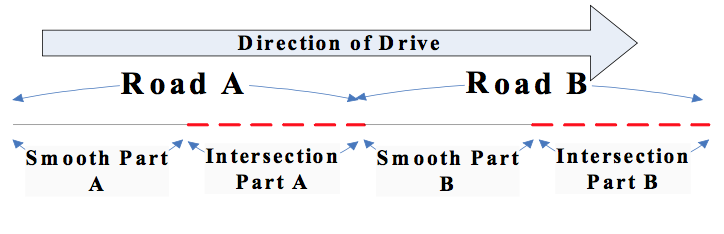
\includegraphics[width=3in]{road_separation}
  \caption{路段分解算法}
  \label{fig:3}
\end{figure}

算法引用自Yue发表在ICCTP 2009的一篇论文中~\cite{yue2009urban}。该算法将道路分成平滑部分(Smooth Part)和路口部分(Intersection Part)。 IP段长度由路由确定,是由道路等级和历史等待队列长度计算得出的。还将两条相邻的路段定义为道路A和道路B,表示为$R_{}A$和$R_{B}$。两个连续的GPS信号分别被定义为$G_{j}(x_{j},y_{j},T_{j})$和$G_{j + 1}(x_{j + 1},y_{j + 1},T_{j + 1})$,其中(x,y)分别是匹配的GPS坐标,而T是相应的时间戳。计算$R_{A}$段行驶速度的公式如下(\ref{f2.2.1})。

\begin{equation}
TS_{A}=\frac{L_{TotalA}}{\frac{L_{intersection}}{TS_{intersection}^{A}}+\frac{L_{TotalA}-L_{intersection}}{TS_{SP}^{A}}}
\label{f2.2.1}
\end{equation}

其中,$TS_{A}$代表道路A的平均速度,分母左右分别为路口路段的时间和平滑路段的时间。$TS_{SP}^{A}$伪平滑路段的速度,使用所有在平滑路段A上前后两殿的平均速度按所占道路比例加权,找不到这样的点则使用该段的瞬时速度代替。$TS_{intersection}^{A}$则是路口路段的速度,使用路口路段车辆平均瞬时速度来计算。这种算法十分依赖瞬时速度,然而我们得到的浮动车GPS数据的瞬时速度经常出现非常大的偏差,所以这种算法也不适合我们的系统。

\subsection{延迟估计算法}

\begin{figure}[H] 
  \centering
  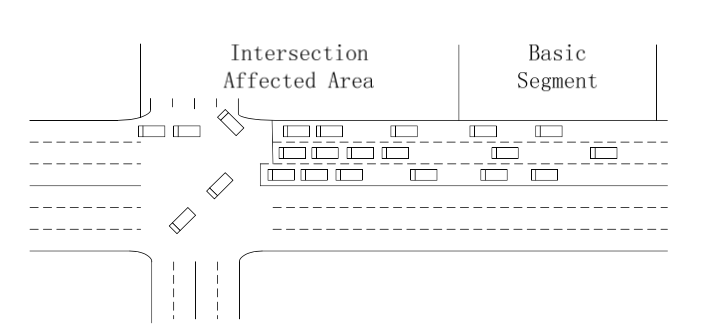
\includegraphics[width=3in]{delay}
  \caption{延迟估计算法}
  \label{fig:4}
\end{figure}

算法引用自Zhao-cheng2014年发表在CICTP的一篇论文中~\cite{he2014delay}。算法的原理是确定路口受影响区域外的两个最近的GPS点,来确定路口行驶时间。在计算路口延迟之前,需要车辆在路口的行驶时间$T_{fcd}$和车辆在加速行驶速度$T_{exp}$的行驶时间。文章中直接采用道路设计速度作为车辆的快速行驶速度。

\begin{figure}[H] 
  \centering
  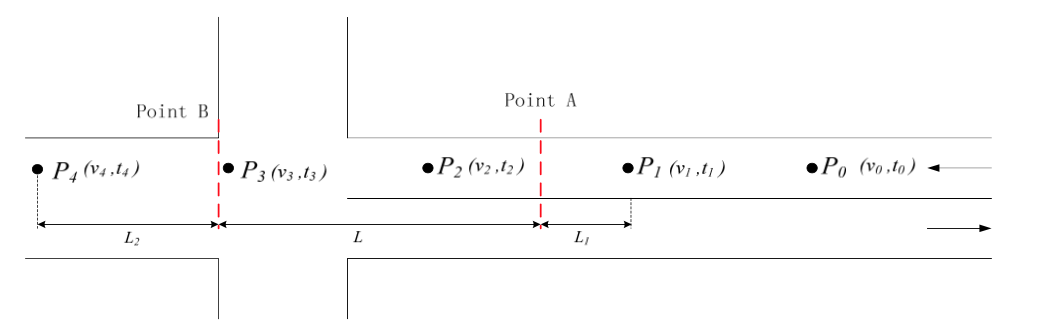
\includegraphics[width=3in]{delay2}
  \caption{计算原理}
  \label{fig:5}
\end{figure}

算法的计算原理见图~\ref{fig:5},其中点A和点B之间的区域是路口影响区域。 假设一个跨越十字路口的出租车轨迹包括几个GPS点$(P_{1},P_{2} ...)$。 选择路口影响区域外的两个最近点(即图~\ref{fig:5}中的$P_{1}$,$P_{4}$)。这两点的速度需要大于零。 点$P_{1}$用于估计进入路口影响区域的车辆的时间戳。 $P_{4}$点则用于估计离开路口影响区域的车辆的时间戳。可以得出如下的公式:

\begin{equation}
t_{A}=t_{1}+\frac{L_{1}}{v_{1}}
\end{equation}

\begin{equation}
t_{B}=t_{4}+\frac{L_{2}}{v_{4}}
\end{equation}

\begin{equation}
T_{fcd}=t_{B}-t_{A}= \left( t_{4}+\frac{L_{2}}{v_{4}}\right) - \left( t_{1}+\frac{L_{1}}{v_{1}}\right)
\end{equation}

参数$v_{1}$,$v_{4}$,$t_{1}$,$t_{4}$是已知的,可以直接通过GPS数据获得。 点$P_{1} $和$P_{4}$的位置可以通过上面的映射对应算法得出。之后就可以计算$L_{1}$,$L_{2}$。 因此,延迟估计的公式如下:

\begin{equation}
D = T_{fcd} - T_{exp} = t_{B} - t_{A} - \frac{L}{v_{exp}}
= \left( t_{4}+\frac{L_{2}}{v_{4}}\right) - \left( t_{1}+\frac{L_{1}}{v_{1}}\right) - \frac{L}{v_{exp}}
\end{equation}

该算法的优势是对于路口的判断很精确,但是需求的数据密度还是相对比较多,需要数据间隔在30s左右,但是我们的数据不能达到这种要求,间隔基本在60s左右,所以这种算法还是无法适用于我们当前的系统。

